\section{Theoretical Analysis}
\label{sec:th_analysis_belief}

In this section, we provide the reader with several results to better grasp the problem of constantly delayed \gls{dmdp}. 
First, we formally prove a fact that is usually taken for granted in the literature: longer delays imply smaller optimal returns.
In the second part, the complexity of constantly delayed \gls{dmdp} will be studied. 
Finally, providing an example, we demonstrate that model-based policy can have sub-optimal performance in some problems.


\subsection{Effect of the Delay on the Performance}
\label{subsec:effect_delay_belief}
For average reward or expected discounted return, it seems reasonable that, all things being equal, the higher the delay of a \gls{dmdp}, the smaller the performance of its optimal policy.
Although natural, this result has not been demonstrated yet. 
We provide a demonstration below. This result requires the following assumption, which ensures that the two processes with different delays are initialised in the same way.

\begin{defi}[Consistent \glspl{dmdp}]
\label{def:consistency_dmdps}
     Let $\delayedmarkovdecisionprocess$ and $\delayedmarkovdecisionprocess'$ be two \glspl{dmdp} with respective delay $\delay$ and $\delay'$ and initial augmented state distributions $\delayeddiscountedstateoccupancydistribution[0][]$ and $\delayeddiscountedstateoccupancydistribution[0][\prime]$.
     If $\delay\le \delay'$, we say that $\delayedmarkovdecisionprocess$ and $\delayedmarkovdecisionprocess'$ are consistent if:
    \begin{align*}
        \probability(S_0=s_0;\delayeddiscountedstateoccupancydistribution[0][])= \probability(S_0=s_0;\delayeddiscountedstateoccupancydistribution[0][\prime]),
    \end{align*}
    and $\forall t\le\delay$, 
    \begin{align*}
        \probability(A_t=a_t;\delayeddiscountedstateoccupancydistribution[0][])= \probability(A_t=a_t;\delayeddiscountedstateoccupancydistribution[0][\prime]).
    \end{align*}
\end{defi}


\begin{thm}
\label{th:perf_delay_vector_all_weight}
    Let $\delayedmarkovdecisionprocess_{1}$ and $\delayedmarkovdecisionprocess_{2}$ be two consistent \glspl{dmdp} with respective delay $\delay_1$ and $\delay_2$.
    Consider $\expectedreturn[1][\star]$ and $\expectedreturn[2][\star]$, their respective optimal expected discounted returns or average reward.
    If $\delay_1<\delay_2$, then one has:
    \begin{align*}
        \expectedreturn[2][\star] \le \expectedreturn[1][\star].
    \end{align*}
\end{thm}
\begin{proof}
    To prove this result, we first show that there is a non-stationary history-based policy in $\delayedmarkovdecisionprocess_{1}$ which has the same augmented state distribution as the optimal Markovian policy in $\delayedmarkovdecisionprocess_{2}$, $\optimalpolicy_2$.
    To define this policy, we divide the trajectory into two periods.
    In the first period, when $t\ge\delay_2$, we note $(s_{t-{\delay_2}},a_{\delay_2},\dots,s_{t-1},a_{t-1},s_t)$ the history of the last $\delay_2$ steps. 
    The agent in $\delayedmarkovdecisionprocess_{2}$ observes the augmented state,
    \begin{align*}
        x_t'=(s_{t-{\delay_2}},a_{t-{\delay_2}},\dots,a_{t-1}).
    \end{align*}
    Since $\delay_1<\delay_2$, the agent in $\delayedmarkovdecisionprocess_{1}$ can observe the following quantity,
    \begin{align*}
        \overline x_t=(s_{t-{\delay_2}},a_{t-{\delay_2}},\dots,s_{t-{\delay_1}},a_{t-{\delay_1}}\dots,a_{t-1}),
    \end{align*}
    which is in $\statespace^{\delay_1-\delay_2}\times\actionspace^{\delay_2}$. 
    Note that this ``state'' includes a history of $\delay_1-\delay_2$ states and actions that would not be used by a Markovian policy in $\delayedmarkovdecisionprocess_{1}$.
    We define our candidate policy $(\pi_t)_{t\ge0}$ for  $t\ge\delay_2$ as follows,
    \begin{align*}
        \pi_t(\cdot\vert\overline x_t) = \optimalpolicy_2(\cdot\vert x_t').
    \end{align*}
    When $\delay_1\le t<\delay_2$, then the agent in $\delayedmarkovdecisionprocess_{1}$ cannot yet observe a $\delay_2$-steps old state.
    However, knowing the initial state distribution $\delayeddiscountedstateoccupancydistribution[0,2][]$ of $\delayedmarkovdecisionprocess_{2}$, one can define the policy as 
    \begin{align*}
        \pi_t(a_t) = \probability(A_t=a_t;\delayeddiscountedstateoccupancydistribution[0,2][]).
    \end{align*}
    Basically, $\pi_t$ ignores the augmented state and selects its action with the same probability as the initial action distribution in $\delayedmarkovdecisionprocess_{\delay_2}$.
    
    We shall now prove that this policy induces the same state distribution in $\delayedmarkovdecisionprocess_{2}$. 
    We note $\delayeddiscountedstateoccupancydistribution[t][\pi]$ the undiscounted state distribution of $(\pi_t)_{t\ge0}$ at time $t$ and $\delayeddiscountedstateoccupancydistribution[t][\optimalpolicy_2]$ that of $\optimalpolicy_2$.
    For $t=\delay_2$, note that,
    \begin{align}
        &\delayeddiscountedstateoccupancydistribution[t][\optimalpolicy_2](x_t')
        \nonumber\\
        &= \delayeddiscountedstateoccupancydistribution[0,2][](s_{t-{\delay_2}},a_{t-{\delay_2}},\dots,a_{t-1})
        \nonumber\\
        &= \delayeddiscountedstateoccupancydistribution[0,1][](s_{t-{\delay_2}},a_{t-{\delay_2}},\dots,a_{t+\delay_1-\delay_2-1})\prod_{i=1}^{\delay_2-\delay_1}\probability(A_{t-i}=a_{t-i};\delayeddiscountedstateoccupancydistribution[0,2][])
        \label{eq:consistency_dmdps}\\
        &=\delayeddiscountedstateoccupancydistribution[0,1][](s_{t-{\delay_2}},a_{t-{\delay_1}},\dots,a_{t+\delay_1-\delay_2-1})\prod_{i=1}^{\delay_2-\delay_1}\pi_{t-i}(a_{t-i})
        \label{eq:def_policy_less_delay}\\
        &\coloneq \delayeddiscountedstateoccupancydistribution[t][\pi](x_t'),\nonumber
    \end{align}
    where \Cref{eq:consistency_dmdps} holds by the assumption of consistency and \Cref{eq:def_policy_less_delay} by the definition of $(\pi_t)_{t\ge0}$ on the first $\delay_2$ steps.
    Then, assuming that $\delayeddiscountedstateoccupancydistribution[t][\optimalpolicy_2]=\delayeddiscountedstateoccupancydistribution[t][\pi]$ for some $t\ge\delay_2$ we shall prove the equality for $t+1$.
    We require some notation to simplify the exposition. First, for $\overline x_t,\overline x_{t+1}\in\statespace^{\delay_1-\delay_2}\times\actionspace^{\delay_2}$, and $a_t\in\actionspace$ we note $\bar{\transitionfunction}(\overline x_{t+1}\vert \overline x_t, a_t) = \probability(X_{t+1}=\overline x_{t+1}\vert X_t=\overline x_t,A_t=a_t)$ the transition probability from pair $(\overline x_t,a_t)$ to $\overline x_{t+1}$. We also define the following measure, for $x_t'\in\statespace\times\actionspace^{\delay_2}$
    \begin{align*}
        \delta_{x_{t}'}(\overline x_{t}) = \delta_{s_{t-\delay_2}'}(s_{t-\delay_2})\prod_{i=1}^{\delay_2}\delta_{a_{t-i}'}(a_{t-i}),
    \end{align*}
    which ensures that the states and action in $x_{t}'$ are contained in $\overline x_{t}$.
    Using this notation, we have,
    \begin{align}
        \delayeddiscountedstateoccupancydistribution[t][\pi](x_{t+1}') 
        &= \int_{\statespace^{\delay_1-\delay_2}\times\actionspace^{\delay_2}} \delayeddiscountedstateoccupancydistribution[t][\pi](\overline x_{t}) \bar{\transitionfunction}(\overline x_{t+1}\vert \overline x_t,a_t) \delta_{x_{t+1}'}(\overline x_{t+1})\pi_t(a_t\vert \overline x_t)\;\de \overline x_t\;\de s_{t-\delay_1+1}
        \nonumber\\
        &= \int_{\statespace^{\delay_1-\delay_2}\times\actionspace^{\delay_2}} \delayeddiscountedstateoccupancydistribution[t][\pi](\overline x_{t}) \bar{\transitionfunction}(\overline x_{t+1}\vert \overline x_t,a_t)
        \delta_{s_{t-\delay_2+1}'}(s_{t-\delay_2+1})\optimalpolicy_2(a_t\vert x_t')
        \nonumber\\
        &\qquad \prod_{i=0}^{\delay_2-1}\delta_{a_{t-i}'}(a_{t-i})\;\de\overline x_t\;\de s_{t-\delay_1+1}
        \nonumber\\
        &= \int_{\statespace^{\delay_1-\delay_2-1}\times\actionspace^{\delay_2+1}} \delayeddiscountedstateoccupancydistribution[t][\pi](\overline x_{t})  \delta_{s_{t-\delay_2+1}'}(s_{t-\delay_2+1})
        \optimalpolicy_2(a_t\vert x_t')
        \prod_{i=0}^{\delay_2-1}\delta_{a_{t-i}'}(a_{t-i})\;\de\overline x_t 
        \label{eq:indpt_delta}
        \\
        &= \int_{\statespace\times\actionspace^{\delay_2}} \delayeddiscountedstateoccupancydistribution[t][\pi](x_{t}') p(s_{t-\delay_2+1}\vert s_{t-\delay_2},a_{t-\delay_2}) \delta_{s_{t-\delay_2+1}'}(s_{t-\delay_2+1})
       \nonumber
       \\
        &\qquad \cdot\optimalpolicy_2(a_t\vert x_t')\prod_{i=0}^{\delay_2-1}\delta_{a_{t-i}'}(a_{t-i})\;\de x_t'
        \label{eq:indpt_delta2}
        \\
        &= \int_{\statespace\times\actionspace^{\delay_2}} \delayeddiscountedstateoccupancydistribution[t][\optimalpolicy_2](x_{t}') \augmentedtransitionfunction(x_{t+1}'\vert x_t',a_t)\optimalpolicy_2(a_t\vert x_t')\;\de x_t'
       \nonumber
       \\
       &= \delayeddiscountedstateoccupancydistribution[t][\optimalpolicy_2](x_{t+1}'),\nonumber
    \end{align}
    where \Cref{eq:indpt_delta} holds since all the terms involved in the Dirac measures $\delta$ are already fixed by $\overline x_t$ and $x_{t+1}'$ and \Cref{eq:indpt_delta2} holds since no term but  $\delayeddiscountedstateoccupancydistribution[t][\pi](\overline x_{t})$ depend on $s_{t-\delay_2+2},\dots,s_{t-\delay_1}$ and we can therefore integrate those terms out.
    
    Summarising, we have found a non-stationary history-based policy in  $\delayedmarkovdecisionprocess_{1}$ which has the same augmented state distribution at any time as the optimal policy in $\delayedmarkovdecisionprocess_{2}$. 
    By design, it selects the same action as $\optimalpolicy_2$ in any state and therefore has the same reward at any time.
    This shows that $(\pi_t)$ and $\optimalpolicy_2$ have the same discounted expected return or average reward.
    Since $(\pi_t)$ is a particular policy for $\delayedmarkovdecisionprocess_{1}$, the optimal policy in $\delayedmarkovdecisionprocess_{1}$ may yield an even higher return or average reward. This concludes the proof.
\end{proof}

\begin{remark}
    From \cite[Theorem~6.2.10 and Theorem~8.1.2]{puterman1994markov} we even know that there is an optimal Markovian (in the sense that it uses only the augmented state and not more history) policy in $\delayedmarkovdecisionprocess_{1}$  that yields $\expectedreturn[1][\star]$.
\end{remark}

We extend the previous result with a corollary, which says that although the policy that we have designed in the proof is history-based, there exists a Markovian policy in $\delayedmarkovdecisionprocess_{1}$ (also in the sense that it uses only the augmented state and not more history) with the same state distribution as the optimal policy in $\delayedmarkovdecisionprocess_{1}$.

\begin{prop}
\label{corol:markov_optimal_delayed_equiv}
    Let $\delayedmarkovdecisionprocess_{1}$ and $\delayedmarkovdecisionprocess_{2}$ be two consistent \glspl{dmdp} with respective delay vectors $\delay_1$ and $\delay_2$ such that $\delay_1<\delay_2$. 
    Consider a Markovian policy $\delayedpolicy_2$ in $\delayedmarkovdecisionprocess_{2}$ (that is, with respect to its augmented state $\augmentedstatespace_2=\statespace\times\actionspace^{\delay_2}$) with $\sigma$-finite occupancy measure.
    Then there exists a Markovian policy in $\delayedmarkovdecisionprocess_{1}$ (with respect to its augmented state $\augmentedstatespace_1=\statespace\times\actionspace^{\delay_1}$) that has the same state-action distribution induced on $\augmentedstatespace_1$ as the optimal policy $\delayedpolicy_2$.
\end{prop}
\begin{proof}
    Let $\delayedpolicy_2$ be a policy with $\sigma$-finite occupancy measure in $\delayedmarkovdecisionprocess_{2}$.
    From the proof of \Cref{th:perf_delay_vector_all_weight}, one can build a history-based policy $\delayedpolicy_1$ in $\delayedmarkovdecisionprocess_{1}$ with the same state-action distribution on $\augmentedstatespace_2$.
    Then, from \cite[Theorem~3]{laroche2022non} one has that there is a Markovian policy $\delayedpolicy$ in $\delayedmarkovdecisionprocess_{1}$ with the same state distribution over $\augmentedstatespace_1$ as this $\delayedpolicy_1$. 
    This concludes the proof.
\end{proof}

\subsection{On the Complexity of Constant Delays}
\label{subsec:delay_complexity}

The following proposition is a direct implication from \cite{bertsekas1987dynamic,altman1992closed} which states that a \gls{dmdp} with state observation and/or action execution delays can be cast back into an \gls{mdp} by using the augmented state.
\begin{prop}
\label{pp:dmdp_pompd}
Model-based and memoryless approaches to state observation or action execution delays cast the problem from a \gls{dmdp} to a \gls{pomdp}. 
In particular, the framework of a policy using belief representations as input can be reduced to POMDPs.
\end{prop}
\begin{proof} 
    From \cite{bertsekas1987dynamic,altman1992closed}, by using the augmented state, a \gls{dmdp} is cast to an \gls{mdp}. 
    Then, since model-based approaches use only some statistic of the current state computed from the augmented state and since the memoryless uses only part of the latter, the observation used by the agent for its policy can be seen as a partial observation of the true augmented state.
    This is exactly the framework of a \gls{pomdp}.
\end{proof}

This result is a negative result as the \gls{dmdp} can be cast into an \gls{mdp} by augmenting the state, but we are now dealing with only a partial observation of it and it is known that \gls{pomdp} can be much harder to solve than \gls{mdp} \cite[Theorem 6]{papadimitriou1987complexity}. 
It is confirmed by \cite[Theorem~2]{walsh2009learning} who show that the problem of planning in a \gls{dmdp} using the augmented state is already NP-Hard. 

\begin{figure}[t]
    \centering
    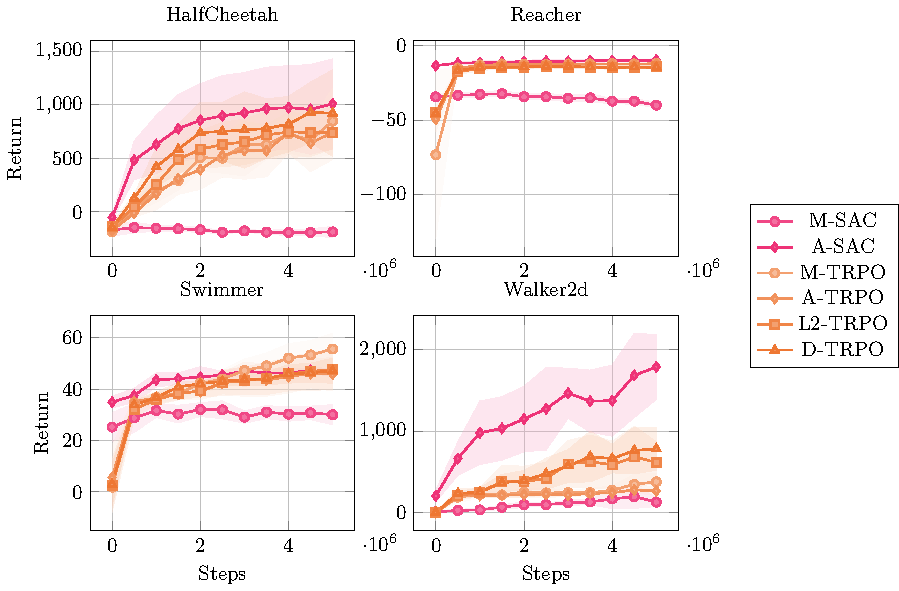
\includegraphics[labelbelief=mdppomdpsets]{img/thesis_plots_belief.pdf}
    \caption{Dimensionality of the problem with respect to the quantity of information that is available to the agent. 
    The trade off between these quantities is symbolised by the black dashed line.
    The undelayed \gls{mdp} ($\textbf{U}$) has complete information and low dimensionality while the augmented state approach ($\textbf{A}$), which is an MDP~\cite{bertsekas1987dynamic,altman1992closed}, has higher dimensionality. 
    Memoryless approach ($\textbf{Me}$) has low dimensionality but is a \glspl{pomdp} as shown in \Cref{pp:dmdp_pompd}.
    Model-based approach ($\textbf{Mo}$) also yields a \glspl{pomdp}~\Cref{pp:dmdp_pompd}. 
    This last method allows to trade off dimensionality and observability.
    } 
\label{fig:relations_dmdp_mdp_pomdp}
\end{figure}



\subsection{Counter Example for Model-Based Approaches}
\label{subsec:model_based_sub_optimal}

Despite the negative result exposed in the previous section, one could hope that the special structure of \gls{dmdp} allows model-based approaches to achieve optimal performance. 
Sadly, we prove in the following proposition that the optimal return over the set of model-based policies can be sub-optimal with respect to the best augmented state-based policy.

\begin{prop}
\label{pp:counter_example_belief_based}
    Let $\expectedreturn[b][*]$ be the optimal return over the space of belief-based policies and $\expectedreturn[a][*]$ the one over the space of augmented state-based policies for the same \gls{dmdp}. Then, there exists \glspl{dmdp} where
    \begin{align*}
        \expectedreturn[b][*]<\expectedreturn[a][*].
    \end{align*}
\end{prop}
\begin{proof}
    We prove this result by giving an example of such a \gls{dmdp}.
    The example is represented in \Cref{fig:counter_example_dmdp_pomdp}. 
    In this example, the delay is set to two steps. The agent starts at the lowermost state, and, to initialise the process, the first two actions are selected uniformly at random. In any state, two actions are available, $a$ and $b$. 
    Note that, except for the uppermost states, no transition yields a reward. 
    The former act as absorbing states and provide a discounted return or average reward that is indicated above the node.
    Therefore, the reward collected by the agent will only depend on the uppermost state that it reaches.
    All the transitions are deterministic, except for the transitions indicated with dashed lines. 
    In the latter case, the probability of following either route is $1/2$.
    The peculiarity of this \gls{mdp} is the following. 
    Due to the 2-step delay, after the initialisation, the agent is either in state $s$ or $s'$.
    This means that, given the structure of the \gls{mdp}, the belief of the agent about its current state is $1/2$ for $s$ and $1/2$ for $s'$.
    Notably, a belief-based policy is blind to the path the agent has taken to reach $s$ or $s'$.
    The first path, in red, goes to the state directly above the initial state deterministically and then transitions to either $s$ or $s'$. 
    The second path, in blue, goes left or right at the first step before transitioning deterministically to either $s$ or $s'$. 
    The interesting property of the blue path is that from the second step, the agent will know whether it is going to reach $s$ or $s'$. 
    However, on the red path, the agent will have to wait for an extra step before knowing whether it actually was in $s$ or $s'$.
    A belief-based agent sees the same state whatever the path that he will follow, while an augmented state-based agent knows whether it will follow the blue or red path from the first action contained in the augmented state.
    The belief-based agent must therefore select an action which optimises the return regardless of the path, while the augmented state-based policy might leverage this additional information to select its actions more carefully. 
    
    The agent has to select the next two actions before achieving the final reward. 
    For the red path, the agent will select the two actions before obtaining any knowledge about whether he will follow the left or right branch. 
    The reward that the agent collects for each combination of actions is given in \Cref{tab:reward_red_path}. 
    Instead, for the blue path, the agent may adapt its second action according to the branch of the \gls{mdp} it is following. 
    Similarly, we provide the rewards given the first action and the observed state in \Cref{tab:reward_blue_path}. 
    Note that given this state and action, the optimal action to choose next is fixed. 
    
    We design the initialisation so that the agent has the same probability of following either path. 
    For the red path, the agent should play $b$ as a first action followed by $a$ to collect a reward of $12.5$. 
    For the blue path, it should instead select first action $a$ and then adapt its second action based on the observation to get an average reward of $15$ compared to an average reward of $12.5$ if it played $b$ as a first action.
    
    Therefore, the augmented state-based policy will follow the above reasoning to collect a reward of $\expectedreturn[a][*]=13.75$ on average. 
    The belief-based policy is instead constrained to select the same action first for both paths as it is unaware of the path it will follow.
    When selecting $a$ first, the agent will get a reward of $10$ in the red path case and $15$ in the blue path case. 
    By selecting $b$ first, it will collect a reward of $6.25$ in the red path case and $12.5$ in the other. 
    This means that, whatever its choice of the first action, it will always collect a smaller reward in expectation. 
    Its best return is obtained by playing $a$ first and amounts to $\expectedreturn[b][*]=12.5$. 
    This concludes the proof.
\end{proof}


\begin{figure}[t]
    \centering
    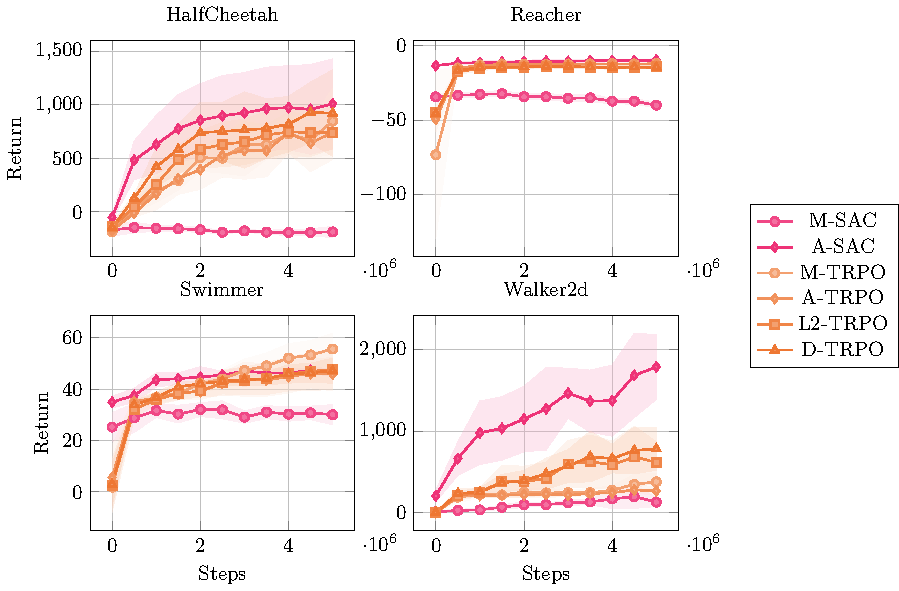
\includegraphics[labelbelief=counterexampledmdppomdp]{img/thesis_plots_belief.pdf}
    \caption{Example of a \gls{dmdp}, where, for a 2-step delay, the belief-based policy is sub-optimal with respect to the best augmented state-based policy.
    In any state, the agent can select either one of two actions, $a$ and $b$.  
    None of the transitions but the uppermost ones provide a reward. For the latter, a recurrent state provides the discounted return or average reward that is indicated above. 
    All transitions are deterministic except for the dashed ones, where the agent selecting the given action has a probability of $1/2$ to follow either one of the edges. 
    The agent starts at the lowermost state. 
    The underlying \gls{mdp} is designed such that it has two paths, which give rise to the same belief over the states $s$ and $s'$.}
    \label{fig:counter_example_dmdp_pomdp}
\end{figure}


\begin{table}[t]
\centering
\begin{tabular}{l|rr} 
  & \multicolumn{1}{c}{$a$} & \multicolumn{1}{c}{$b$} \\ 
\hline
$a$ & $5$ & $10$ \\ 
$b$ & $12.5$ & $0$ \\
\end{tabular}
\caption{\label{tab:reward_red_path}Rewards for all couples of first (row) and second (column) actions, initially following the red path.}
\end{table}

\begin{table}[t]
\centering
\begin{tabular}{l|rr} 
  & \multicolumn{1}{c}{$s$} & \multicolumn{1}{c}{$s'$} \\ 
\hline
$a$ & $a\rightarrow10$ & $b\rightarrow20$ \\ 
$b$ & $a\rightarrow15$ & $a\rightarrow10$ \\
\end{tabular}
\caption{\label{tab:reward_blue_path}Rewards for all couples of first action (row) and state observed at the next step (row), initially following the blue path. The second action is selected optimally and indicated inside the table.}
\end{table}

However discouraging this counter-example can be, we provide in \Cref{sec:th_analysis_imitation} an analysis of a special type of belief-based policy and show that, under smoothness conditions, the return of this policy is close to the optimal delayed one--up to a constant. 
